% ==============================================================
% SECCIÓN 2: MARCO TEÓRICO — FCS-M2PC
% ==============================================================

% --- Slide 5: Modelo del motor ---
\begin{frame}{Modelo del Motor BLDC en $\alpha\beta$}
    Dinámica eléctrica en el marco estacionario de Clarke:
    \begin{equation}
        \frac{d}{dt}\begin{bmatrix} i_\alpha \\ i_\beta \end{bmatrix} 
        = \frac{1}{L}\left(
            \begin{bmatrix} u_\alpha \\ u_\beta \end{bmatrix}
            - R \begin{bmatrix} i_\alpha \\ i_\beta \end{bmatrix}
            - \begin{bmatrix} e_\alpha(\theta_e) \\ e_\beta(\theta_e) \end{bmatrix}
        \right)
    \end{equation}
    
    donde la BEMF depende de la forma de onda \textbf{shape} $\mathbf{s}(\theta_e)$:
    \begin{equation}
        \mathbf{e}_{\alpha\beta}(\theta_e) = K_e \cdot \omega_m \cdot \mathbf{s}(\theta_e)
    \end{equation}
    
    \begin{itemize}
        \item Si $\mathbf{s}(\theta_e) = [\sin\theta_e,\; -\cos\theta_e]^T$ $\rightarrow$ motor senoidal ideal
        \item Motor real: $\mathbf{s}(\theta_e)$ contiene armónicos 5to, 7mo, 11vo...
        \item \textbf{El conocimiento preciso de $\mathbf{s}(\theta_e)$ es clave} para generar referencias de corriente que produzcan torque constante.
    \end{itemize}
\end{frame}

% --- Slide 6: FCS-M2PC ---
\begin{frame}{FCS-M2PC: Control Predictivo con Dos Vectores por Período}
    \textbf{Idea clave} (Coronado-Andrade et al., 2025): dividir $T_s$ en sub-intervalos y aplicar \textbf{combinaciones} de dos vectores activos + vector nulo.
    
    \vspace{0.2cm}
    
    \begin{columns}[T]
    \begin{column}{0.55\textwidth}
        Predicción de corriente al fin del período:
        \begin{equation}
            \mathbf{i}(k{+}1) = \mathbf{i}(k) + \mathbf{f}_1 t_1 + \mathbf{f}_2 t_2 + \mathbf{f}_0 t_0
        \end{equation}
        donde $\mathbf{f}_j = \frac{1}{L}(\mathbf{u}_j - \mathbf{e} - R\mathbf{i})$ y $t_1+t_2+t_0 = T_s$.
        
        \vspace{0.3cm}
        
        Función de costo:
        \begin{equation}
            g^* = \min_{t_1, t_2} \left\| \mathbf{i}^*_{\text{ref}}(k{+}1) - \mathbf{i}_{\text{pred}}(k{+}1) \right\|^2
        \end{equation}
        
        \vspace{0.2cm}
        \textbf{Ventaja vs.\ FCS-MPC clásico:} reducción de 75--80\% en RMSE de corriente \citep{coronado2025}.
    \end{column}
    \begin{column}{0.42\textwidth}
    \centering
    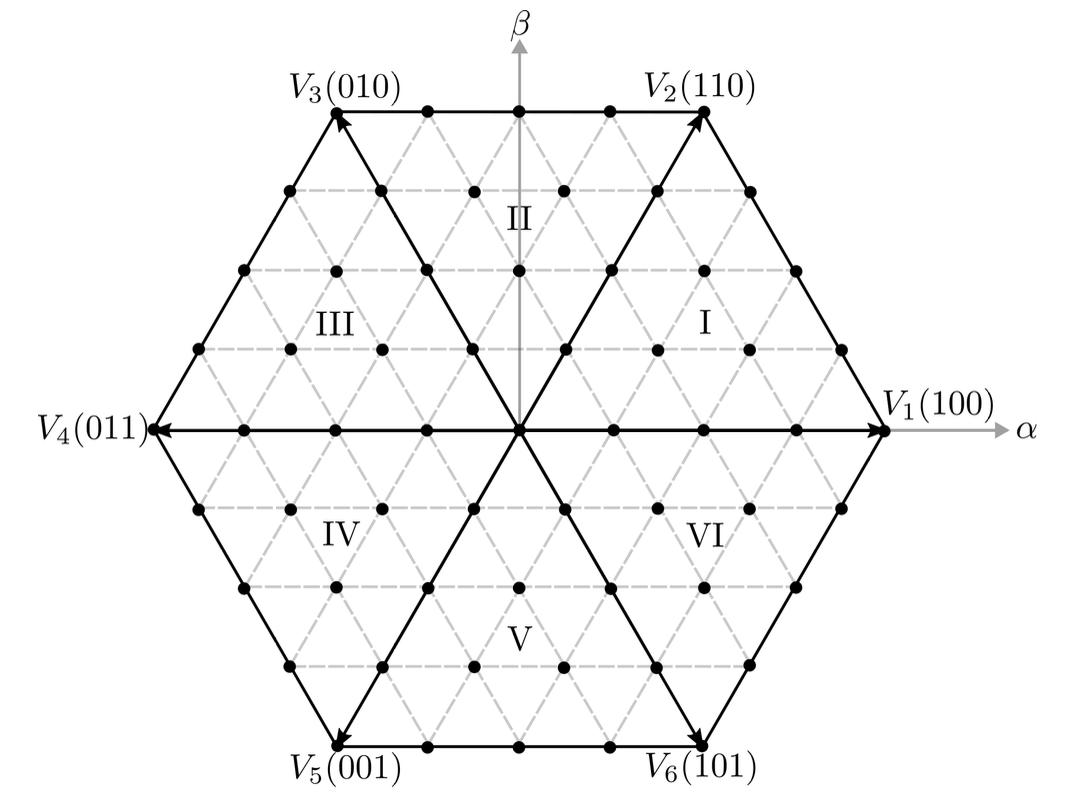
\includegraphics[width=0.95\linewidth]{fig/m2pc_vector_diagram.png}
    {\footnotesize Diagrama vectores de voltaje}
    \end{column}
    \end{columns}
\end{frame}

% --- Slide 7: El rol de la BEMF en el M2PC ---
\begin{frame}{¿Por Qué la BEMF Importa Tanto en el M2PC?}
    La BEMF aparece en \textbf{dos lugares críticos}:
    
    \vspace{0.3cm}
    
    \begin{columns}[T]
    \begin{column}{0.48\textwidth}
        \begin{block}{1. Generación de $\mathbf{i}^*_{\text{ref}}$}
            Para torque constante $T_{\text{ref}}$:
            \begin{equation}
                \mathbf{i}^* = \frac{T_{\text{ref}}}{K_t \|\mathbf{s}\|^2} \cdot \mathbf{s}(\theta_e)
            \end{equation}
            Si $\mathbf{s}$ es incorrecto $\rightarrow$ la referencia tiene armónicos $\rightarrow$ torque oscila.
        \end{block}
    \end{column}
    \begin{column}{0.48\textwidth}
        \begin{block}{2. Modelo de predicción}
            \begin{equation}
                \mathbf{i}_{\text{pred}} = \mathbf{i} + \frac{T_s}{L}(\mathbf{u} - \hat{\mathbf{e}} - R\mathbf{i})
            \end{equation}
            Si $\hat{\mathbf{e}} \neq \mathbf{e}_{\text{real}}$ $\rightarrow$ predicción sesgada $\rightarrow$ vector de voltaje subóptimo.
        \end{block}
    \end{column}
    \end{columns}
    
    \vspace{0.5cm}
    
    \begin{center}
        \fcolorbox{red}{red!5}{\parbox{0.85\textwidth}{\centering
            \textbf{Conclusión:} Un modelo preciso de $\mathbf{s}(\theta_e)$ mejora \textit{simultáneamente} la referencia y la predicción.\\
            $\rightarrow$ Motivación para aprender $\mathbf{s}(\theta_e)$ del motor real.
        }}
    \end{center}
\end{frame}